% To compile:
%   pdflatex introDS.tex
%   makeindex introDS.idx
%   pdflatex introDS.tex
\documentclass[11pt]{book}
\usepackage[usenames,dvipsnames]{color}
\usepackage{bbding}  % for checkmark and X
\usepackage{array}           % For double-column exercises.
\usepackage{longtable}       % For double-column exercises.
\usepackage[normalem]{ulem}  % For strikethrough.
\usepackage{paralist}
\usepackage{enumitem}        % To "resume" enumerated lists.
\usepackage{epsfig}
\usepackage[nokeyprefix]{refstyle}
\usepackage{afterpage}
\usepackage{aurical}
\usepackage[T1]{fontenc}
\usepackage{varwidth}
\usepackage{multicol}
\usepackage{fancybox}
\usepackage[makeidx]{hvindex}
\usepackage{textcomp}
\usepackage{fancyvrb}
\usepackage{footnote}
\usepackage{makecell}
\usepackage{amsmath,amsthm,amsfonts,amssymb,latexsym}
\usepackage{MnSymbol}
\usepackage{wasysym}
\usepackage{float}
\usepackage{wrapfig}
\usepackage{upquote}
\usepackage[hidelinks]{hyperref}
\usepackage[width=.9\textwidth,singlelinecheck=true,skip=1pt,font=small,labelfont=bf]{caption}

\newcommand{\freakingtilde}{\raisebox{0.5ex}{\texttildelow}}

\makesavenoteenv{tabular}  % to allow footnotes in tables
\makesavenoteenv{figure}  % to allow footnotes in tables

\definecolor{darkgreen}{rgb}{0,.55,0}
\definecolor{darkred}{rgb}{.75,0,0}


%\captionsetup{width=.9\textwidth}

%\usepackage{enumerate}

% Crazy macro from:
% https://tex.stackexchange.com/questions/36401/drawing-boxes-around-words
% Used in "discovering" chapter.
\def\bluebox#1{\leavevmode \setbox0=\hbox{#1}%
   \dimen0=\wd0 \edef\posxA{\expandafter\ignorept\the\dimen0 \space}%
   \hbox{\kern3pt\pdfliteral{q .8 .8 1 rg .8 .8 1 RG .9963 0 0 .9963 0 0 cm 1
j 1 J 6 w
                             0 0 m 0 5 l \posxA 5 l \posxA 0 l 0 0 l B Q}%
         \box0 \kern3pt}%
}
{\lccode`\?=`\p \lccode`\!=`\t  \lowercase{\gdef\ignorept#1?!{#1}}}

\makeindex

\newenvironment{custommargins}[2]%
  {\addtolength{\leftskip}{#1}\addtolength{\rightskip}{#2}}{\par}

% Set left margin - The default is 1 inch, so the following
% command sets a 2-inch left margin.
\setlength{\oddsidemargin}{1in}
\setlength{\evensidemargin}{0in}
% Set width of the text - What is left will be the right margin.
% In this case, right margin is 8.5in - 1.25in - 6in = 1.25in.
\setlength{\textwidth}{5.5in}

% Set top margin - The default is 1 inch, so the following
% command sets a 0.75-inch top margin.
\setlength{\topmargin}{.75in}

% Set height of the text - What is left will be the bottom margin.
% In this case, bottom margin is 11in - 0.75in - 9.5in = 0.75in
\setlength{\textheight}{7.25in}

\setlength{\parindent}{0pt}
\setlength{\baselineskip}{1.5pt}
\setlength{\parskip}{6pt}

\begin{document}

\title{{\Huge Introduction to the Science of Data}\\DATA 101 lecture notes\\
{\small version 1.0}}
\author{Stephen Davies, Ph.D.\\Computer Science Department\\University of Mary Washington}
\date{}
\maketitle


\thispagestyle{empty}

Copyright \textcopyright \ 2020 Stephen Davies.

\bigskip

University of Mary Washington\\
Department of Computer Science\\
Trinkle Hall\\
1301 College Avenue\\
Fredericksburg, VA  22401

\vspace{.4in}

Permission is granted to copy, distribute, transmit and adapt this work under a
Creative Commons Attribution-ShareAlike 4.0 International License:

\vspace{-.2in}
\begin{center}

\includegraphics{cc_license.png}\\
\smallskip
\url{http://creativecommons.org/licenses/by-sa/4.0/}
\end{center}

\vspace{.1in}
If you are interested in distributing a commercial version of this work, please
contact the author at \texttt{stephen@umw.edu}.

\vspace{1.6in}
The \LaTeX source for this book is available from:
\url{https://github.com/rockladyeagles/crystal-ball-1}.

\vspace{.4in}
Cover art copyright \textcopyright \ 2020 Elizabeth M.~Davies.

\frontmatter

\renewcommand{\contentsname}{Contents}

\setcounter{tocdepth}{0}
\tableofcontents

%\include{preface}

\setcounter{chapter}{0}

\mainmatter

\chapter{Introduction}
\label{ch:intro}

If this marks your first exposure to the new and exciting discipline of
\textit{data science}, you occupy an enviable position. Still in front of you
is all the cool stuff, even the first few sparks of magic when you learn how to
plug data into electrical sockets, perform automated prediction, and write the
first gems of code to probe the depths of an interesting data set. I'm a bit
jealous, tbh, but am also excited to explore it all again with you, which is
the next best thing!

This field has changed the world like hardly any other has, and on an
incredibly short time scale, too. Just a couple decades ago, businesses and
organizations were routinely making major decisions based on gut feelings and
anecdotal observations. Doctors eyeballed sets of symptoms and diagnosed
patients largely based on what conditions they themselves had seen before, or
seen recently. Online sellers gave product recommendations that made sense to
\textit{them}, completely missing patterns and trends that would become
apparent if the characteristics and purchasing patterns of past customers were
taken into account.

Part of the reason decision makers made these suboptimal choices was because it
wasn't yet clear how much punch data science would pack. Another reason was
that the technology wasn't there yet: the processing power and storage capacity
to work with extremely large data sets wasn't commonly available, and of course
the data itself hadn't all been gathered yet. No more! All these parts are here
now. And somewhat incredibly, they're all at your disposal for low (or even no)
cost.

\textbf{This is the era of data science.} If you want to understand and make an
impact on your world, I can honestly think of no better field to dive into than
this one, no matter what your sphere of interest. The ability to command these
techniques and tools gives you both great insight and great power to influence
how life on planet Earth proceeds from this day forward.

\section{Defining Data Science}

\index{data-to-wisdom hierarchy}

\label{dsDefinition}
When people ask me what data science \textit{is}, here's my go-to definition:
\textbf{deriving knowledge from data}. But interpreting that phrase entails
dissecting the difference between ``knowledge'' and ``data,'' two related but
different terms. And that brings me to the \textbf{data-to-wisdom hierarchy},
depicted in Figure~\ref{dataHierarchy}. Let's break it down.

\begin{figure}[ht]
\centering
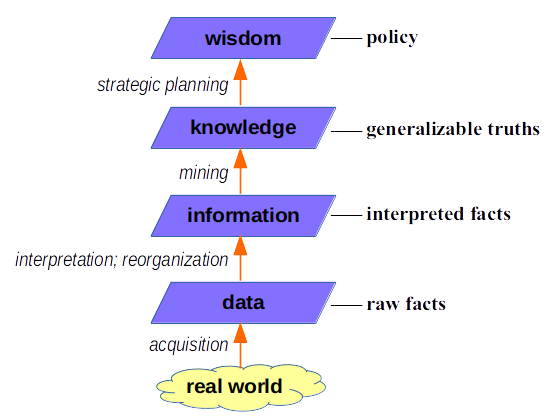
\includegraphics[width=0.9\textwidth]{dataHierarchy.png}
\caption{The data-to-wisdom hierarchy.}
\label{dataHierarchy}
\end{figure}

\subsection{The real world}
\index{real world}
\index{acquisition}

Ultimately, what we're interested in is not data, but aspects of the
\textbf{real world} -- album sales and video views, stock prices and employment
rates, hurricane trajectories and virus hot spots, or whatever. Data science
can't really get off the ground until some sort of \textbf{data acquisition}
takes place that records measurements of the real world in electronic form.

This sounds obvious, but it's important to keep in mind, actually. No matter
how much time we spend working with data, \textit{it's never the data that
actually matters -- it's the real-world phenomenon the data represents.} It
might seem strange to say that ``data'' is merely incidental to a data
scientist, but it's true. And I've definitely seen more than one data scientist
get so locked on to the data that they forget this basic truth.

One important observation is that decisions about exactly \textit{which} data
to acquire from the real world are often crucial in how things are interpreted
later on. To take an example close to home, let's say we're gathering
information on college professors so we can gauge which universities have the
highest performing faculty, and how this might be changing over the years. We
choose some representative set of criteria to measure for each faculty member
to get a rough assessment of their performance. Let's say we choose three
things: the number of research papers the professor publishes each year, the
total amount of research funding they've been granted, and the average student
evaluation score of the courses they teach. That seems like a good first cut at
assessing ``faculty performance.'' We then go on our merry data science way,
finding correlations, making data visualizations, and drawing conclusions.

This is all fine and dandy, provided we always keep in mind that it was those
three qualities, and \textit{only} those three, that we gathered in the first
place. If our study gains any traction, and university professors find they
have a vested interest in being ranked high in our yearly study, we'll discover
that they act to maximize \textit{only} the categories that are being
collected. We didn't gather data on how many university committees they served
on, or how many independent studies they supervised, or how many advisees they
had, \textit{etc.} Those metrics will inevitably become minimized in
importance, because they weren't part of what we lifted out of the real world
and onto the bottom rung of our lofty chain.

\index{GDP}
\index{Dow Jones Industrial Average}
\index{stock market}

The moral is: what we measure matters, often more than we realize. Our
country's GDP and the Dow Jones Industrial Average are easy things to quantify,
and so we often do. And thus they gain great importance in analyses of the
economy. But are they actually the most important indicators? Does focusing on
them leave out other, perhaps more vital, benchmarks? I'll just leave you with
that question for now.

\subsection{Data}

\index{gobbledy-gook}
\index{data}
\index{interpretation}

Have you ever gotten blood work done, say for an annual physical? I have. I
like to look over the numbers when the doctor hands me the results, just to
chuckle and wonder what they all mean. To me, a non-physician, they're all
pretty much gobbledy-gook. They tell me my TBC is 4.93 x10E6/$\mu$L, that
I have 5.7 Absolute Neutrophils, and a slightly out-of-range NT-proBNP (just
53.49 pg/mL, whatever the heck that means).

When I use the word \textbf{data} in the context of the hierarchy, this is what
I mean: recorded measurements, often (but not always) quantitative, that have
not yet been \textbf{interpreted}. They may be very precise, but they're also
quite meaningless without the context in which to understand them. They'd even
be meaningless to a \textit{physician} if I didn't provide the labels; try
telling your doctor that you have 4.93 ``something'' and see whether he/she
freaks out.

The good news is that when we're at the data stage of the hierarchy, we at
least have the stuff in an electronic form so we can start to \textit{do}
something with it. We also often make choices at this stage about how to
\textbf{organize} the data, choosing the appropriate type of atomic and/or
aggregate data structures that we'll discuss in detail in
Chapters~\ref{ch:atomicData} and beyond. This will allow us to bring our
analysis equipment to bear on the problem in powerful ways.

\subsection{Information}
\index{information}

Data becomes \textbf{information} when it \textit{informs} us of something;
\textit{i.e.}, when we know what it means. Getting large amounts of data
organized, formatted, and labeled the right way are jobs for the data
scientist, since turning that morass into useful knowledge is impossible
without those steps. When the aspects of the real world that we've collected
are properly structured and conceptually meaningful, we're in business.


\subsection{Knowledge}
\index{knowledge}
\index{generalizable truths}

Now \textbf{knowledge} is where the real action is. As shown in
Figure~\ref{dataHierarchy}, knowledge consists of \textit{generalizable}
truths.

\index{Chandra}
\index{Austin}
\index{bank teller}

Here's what I mean. Information is about specific individuals or occurrences.
When we say ``Chandra is a female bank teller, and earns \$48,000 a year,'' or
``Austin is a male bank teller, and earns \$69,000 a year,'' we have in our
information repository some individual facts. They can be looked up and
consulted when necessary, as you'll learn in the first part of this book.

But if we say ``women make less money than men do, even at the same jobs,''
we're in a different realm entirely. We have now generalized from specific
facts to more wide-reaching tendencies. In the language of our discipline,
we've moved from information to knowledge.

Properly gleaning knowledge from information is a trickier business than
interpreting individual data points. There are established rules, some of them
mathematical, for determining when an apparent pattern is actually reliable,
what kinds of relationships can be detected with data, whether a relationship
is causal, and so forth. We'll build some important foundations with this kind
of reasoning in this \textit{Crystal Ball} volume and its follow-on companion.
For now, I only want to make the point that \textit{knowledge} -- as opposed to
mere information -- opens up a whole new world of understanding. No longer is
the world limited to a chaotic collection of individual observations: we can
now begin to understand the general ways in which the world works...and perhaps
even to change them.

\subsection{Wisdom}
\index{wisdom}

\textbf{Wisdom} is the gold standard. It represents what we \textit{do} with
our knowledge. Let's say we indeed determine that on average men are paid
higher than women in our country, even for the same jobs. What do we do with
that realization? Is it okay? Do we want to try and fix it, and if so, how?
With laws? Education? Government subsidies? Revolution?

\index{simulation}
\index{uncertainty}

You'll remember my definition of Data Science on p.~\pageref{dsDefinition}:
deriving \textit{knowledge} from \textit{data}. This implies that the
``wisdom'' level of the hierarchy is really outside the discipline, and belongs
to other disciplines instead. And that's partially true: in some sense, the
data scientist's job stops when the deep truths about the real world are
ferreted out and illustrated, leaving it to CEOs, directors, and other policy
makers to act on them. But the data scientist is often involved here too, for a
simple reason: a decision maker wants to know what's likely to \textit{happen}
if a particular policy is implemented. Most non-trivial interventions will have
results that are hard to predict in advance, as well as unintended side
effects. One set of tools in the data scientist's toolkit is for making
principled, calculated predictions about such things, as well as quantifying
the level of \textbf{uncertainty} in the predictions. Sometimes, the technique
of \textbf{simulation} is used -- carrying out experiments on virtual societies
or systems to see the likely aggregate effects of different interventions. It's
like having a high-dimensional, multi-faceted crystal ball that lets you play
out various scenarios to their logical conclusions.

\bigskip

Starting with the rough and tumble real world and helping produce wise
decisions about how humankind can deal with it all: that's the grand promise of
the data science enterprise. And those are the mighty waters you're about to
dip your toes in! I hope you'll find it as exhilarating as I do.

% TODO: Applications (sports, Netflix, image recognition, Google, NLP,
% Coronavirus)


\section{A word of warning}

\index{Spiderman}

Before we dive into the nitty gritty, let me leave you with one more general
thought. It's actually an application of something Spiderman once said: ``with
great power comes great responsibility.''

\index{walking on water}

Here's the deal. The skills you'll learn in this book are so powerful and
(still!) so rare, that when you demonstrate them, people will think you can
walk on water. If you continue in the discipline, you'll become highly
sought-after (and well paid). People will constantly be asking you to work
with new data, to produce plots, predictions, and insights, and basically to do
your magic. You'll be treated as a guru: the oracle people go to when they want
the scoop.

This is ultra-cool, but also dangerous. Why dangerous? One simple reason:
because \textit{when you make a data-related claim, \textbf{people will believe
you.}} Pretty much unquestioningly. Most of your colleagues won't have the
expertise or understanding to double-check your snazzy results. And it wouldn't
occur to them to do that anyway -- after all, you're the wizard.

\index{uncertainty}

The truth of the matter is that data science lives on the knife edge of
\textbf{uncertainty}. With our crystal ball, we can make non-obvious assertions
about the past or present and even predict the future, but as with all
``knowledge,'' we must always hold it tentatively. We may be 95\% confident
that men are paid more than women...but that's only 95\% confidence, not 100\%.
We may have reason to believe that raising the minimum wage in a city will
decrease poverty by 3\%...but there's a 1 in 20 chance that it might decrease
it by as much as 6\%, or even \textit{increase} it by 1\%.

The abiding principle is that you should always be forthright about the limits
of your bold claims, the caveats behind your beautiful plots, and the level of
likelihood that your hypotheses will turn out to be wrong. Admittedly, doing so
will make you seem a little less magic. There are lots of talking heads on
television who deliberately \textit{obscure} the level of uncertainty in their
analyses so that they seem more certain (and more impressive) than they really
are. To be responsible data scientists, though, we're going to do the Spiderman
thing and be up front and transparent about exactly what we've found, and what
we might be missing.

Believe me, this will make you powerful enough!


% Other stuff I mentioned in class:
%
% For math, you think holistically. For programming, you think sequentially /
%   algorithmically.

\chapter{Three kinds of atomic data}
\label{ch:atomicData}

\section{Atomic data}

\index{atomic}
\index{indivisible}
When we say that some data is ``\textbf{atomic},'' we don't mean it's
radioactive; we mean it's \textit{indivisible}.

\index{Democritus}
\index{apple}
The ancients spoke of ``atoms'' as the smallest possible bits of matter. If you
divide up any physical object -- say, an apple -- into parts, you get its
components: a stalk, a stem, skin, seeds, and the sweet juicy stuff. Cut up any
of \textit{those} pieces with a knife and you get smaller pieces. If you
continue to split and split and split, philosophers like Democritus reasoned,
you'll eventually get to tiny indivisible bits that cannot be further
dissected. This is where the physical world bottoms out at the finest degree of
granularity.

Similarly, a piece of atomic data is typically treated as an entire unit, not
as something with internal structure that can be broken down. In the next
chapter we'll learn about various ways that these atoms of data can be strung
together and organized into larger wholes; for now, though, we're just looking
at the atoms themselves.

\section{Environments and variables}

\label{sec:envsAndVariables}
\index{environment}
\index{variable}
\index{variable!name}
\index{variable!value}
A data analysis program -- of which we will write many in this course -- makes
use of an \textbf{environment} as it runs. ``Environment'' just means ``all the
data that is currently in view, and which the program can
access.''\footnote{Confusingly, this use of the term ``environment'' is
different from the term ``programming environment'' I introduced on
p.\pageref{programmingEnvironment}.}  The environment consists of
\textbf{variables}, each of which (usually) has a \textbf{name} and a
\textbf{value}. For example, we might have a variable named \texttt{age} whose
value is 21, and a variable named \texttt{slogan} whose value is
\texttt{"Finger lickin' good"}.

\index{variable!name}
Each variable in the environment must have a \textit{distinct} name
(\textit{i.e.}, no two variables can share the same name). Also, importantly,
the reason these building blocks are called ``variables'' is that their value
can \textit{change} as the program executes. Although we may initially create
an \texttt{age} variable with the value \texttt{21}, later on in the program
the variable's value might change to \texttt{22}, or \texttt{50}, or
\texttt{0}. The variable's \textit{name} never changes, though.

\section{Atomic data types}

\index{variable!type}
There's one other thing that a variable has in addition to its name and value:
a \textbf{type}.\footnote{Strictly speaking, although in languages like Java
variables indeed have types, in Python the \textit{values} have types, not the
variables. This distinction will never be important for us though.}  In a
programming language like Python, every piece of data has a specific type,
which is necessary for determining how it behaves and what all you can do to
it. A question you should ask yourself a lot is: ``okay, I've got a variable in
my environment called \texttt{x}...now what is its type?'' You might have
guessed (correctly) that our \texttt{age} and \texttt{slogan} variables from
the previous section are of different types: one is a number, and the other is
a phrase.

In this course, we'll principally deal with three types of atomic data, all of
which will be familiar to you.


\subsection{Whole numbers}

\index{variable!whole number}
\index{whole number}
\index{likes@``likes''}
\index{votes}
One very common type of data is whole numbers, or integers. These are usually
positive, but can be negative, and have no decimal point. Things like a
person's birth year, a candidate's vote total, or a social media post's number
of ``likes'' are represented with this data type.


\subsection{Real (fractional) numbers}

\index{variable!real number}
\index{real number}
\index{fractional number}
\index{Facebook}
\index{movie rating}
\index{interest rate}
\index{temperature}
You may remember from high school math that the so-called ``real numbers''
include not only integers, but also numbers with digits after the decimal
point. This type can therefore be used to store interest rates, temperature
readings, and average movie ratings on a 1-to-5 scale.

Since all whole numbers are themselves real numbers, you might wonder why we
bother to define two different types for these. Why not just give both kinds of
variables the same real number type? Basically, the answer is that something
``feels wrong'' about that to the Data Science community. A Facebook user might
have 240 friends, or 241, but it would never make sense for her to have 240.3
friends. A consensus has thus arisen: variables that would only ever store
whole numbers really ought to be of a type that's devoted to only whole
numbers. You can violate this convention, but you'll be thought weird by your
fellow developers if you do so.


\subsection{Text}

\index{text}
\index{variable!text}
Lastly, some values obviously aren't numeric at all, like a customer's name, a
show title, or a tweet. So our third type of data is textual. Variables of this
type have a sequence of characters as values. These characters are most often
English letters, but can also include spaces, punctuation, and characters from
other alphabets.

\index{atomic}
\index{Avengers: Endgame@\textit{Avengers: Endgame}}
By the way, this third data type can tiptoe right up to the ``atomic'' line and
sometimes cross it. In other words, we will occasionally work with text values
\textit{non}-atomically, by splitting them up into their constituent words or
even letters. Most of the time, though, we'll treat a character sequence like
\texttt{"Avengers:\ Endgame"} as a single, indivisible chunk of data in the
same way we treat a number like \texttt{42}.

\subsection{But what about...?}

\index{song file}
\index{image file}
\index{video file}
What about other things a computer can store: images, song files, videos? It
turns out that through clever tricks, all these kinds of media and more can be
boiled down to a large number of integers, and stored in an aggregate data
structure like those discussed in the next chapter. At the atomic level, we'll
really only ever need to deal with the three types of this section.

\section{The three kinds in Python}

\index{language-general}
Now the three kinds of atomic data described above are
\textbf{language-general}: this means that they're conceptual, not tied to any
specific programming language or analysis tool. \textit{Any} technology used
for Data Science will have the ability to deal with those three basic types.
The specific ways they do so will differ somewhat from language to language.
Let's learn about how Python implements them.

\subsection{Whole numbers: \texttt{int}}

\index{int@\texttt{int}}
\index{integer}
One of the most basic Python data types is the ``\texttt{int},'' which stands
for ``integer.'' It's what we use to represent whole numbers.

\index{variable!value}
In Python, you create a variable by simply typing its name, an equals sign, and
then its initial value, like so:

\begin{Verbatim}[fontsize=\small,samepage=true,frame=single,framesep=3mm]
revolution = 1776
\end{Verbatim}

\index{line of code}
\index{code}
\index{executing@executing (code)}
\index{statement}
This is our first \textbf{line of code}\footnote{By the way, the word
\textbf{code} is grammatically a mass noun, not a count noun. Hence it is
proper to say ``I wrote some code last night,'' not ``I wrote some codes last
night.'' If you misuse this, it will brand you as a newbie right away.}. As
we'll see, lines of code are \textbf{executed} one by one -- there is a time
before, and a time after, each line is actually carried out. This will turn out
to be very important. (Oh, and a ``line of code'' is sometimes also called a
\textbf{statement}.)


\index{variable!name}
\index{underscore}
Python variable names can be as long as you like, provided they consist only of
upper and lower case letters, digits, and underscores. (You do have to be
consistent with your capitalization and your spelling: you can't call a
variable \texttt{Movie} in one line of code and \texttt{movie} in another.)
Underscores are often used as pseudo-spaces, but no other weird punctuation
marks are allowed in a variable's name.\footnote{Oh, and another rule: a
variable name can't \textit{start} with a digit. So \texttt{r2d2} is a legal
variable name, but not \texttt{007bond}.}

\index{movie rating}
\index{revolution@\texttt{revolution}}
And while we're on the subject, let me encourage you to \textit{name your
variables well}. This means that each variable name should reflect
\textit{exactly} what the value that it stores represents. Example: if a
variable is meant to store the rating (in ``stars'') that an IMDB user gave to
a movie, don't name it \texttt{movie}. Name it \texttt{rating}. (Or even
better, \texttt{movie\_rating}.) Trust me: when you're working on a complex
program, there's enough hard stuff to think about without confusing yourself
(and your colleagues) by close-but-not-exact variable names.\footnote{And I
fully own up to the fact that the \texttt{revolution} variable isn't named very
well. I chose it to make a different point shortly.}

\index{variable!type}
Now remember that a variable has three things -- a name, value, and type. The
first two explicitly appear in the line of code itself. As for the type, how
does Python know that \texttt{revolution} should be an ``\texttt{int}?''
Simple: it's \textit{a number with no decimal point.}

As a sanity check, we can ask Python to tell us the variable's type explicitly,
by writing this code:

\index{type@\texttt{type()}}
\label{typeFunction}
\begin{Verbatim}[fontsize=\small,samepage=true,frame=single,framesep=3mm]
type(revolution)
\end{Verbatim}

If this line of code is executed after the previous one is executed, Python
responds with:

\begin{Verbatim}[fontsize=\small,samepage=true,frame=leftline,framesep=5mm,framerule=1mm]
int
\end{Verbatim}

So there you go.

\index{code snippet}
\index{snippet}
Here's another ``\textbf{code snippet}'' (a term that just means ``some lines
of code I'm focusing on, which are generally only part of a larger program''):

\begin{Verbatim}[fontsize=\small,samepage=true,frame=single,framesep=3mm]
revolution = 1776
moon_landing = 1969
revolution = 1917
\end{Verbatim}

\index{revolution@\texttt{revolution}}
Now if this were a math class, that set of equations would be nonsensical. How
could the same variable (\texttt{revolution}) have two contradictory values?
But in a \textit{program}, this is perfectly legit: it just means that
immediately after the first line of code executes, \texttt{revolution} has the
value \texttt{1776}, and moments later, after the third line executes, its
value has changed to \texttt{1917}. Its value depends entirely on ``where the
program is'' during its execution.

\subsection{Real (fractional) numbers: \texttt{float}}

\index{float@\texttt{float}}
The only odd thing about the second data type in Python is its name. In some
other universe it might have been called a ``real'' or a ``decimal'' or a
``fractional'' variable, but for some bizarre historical reasons it is called a
\texttt{float}.\footnote{If you're curious, this is because in computer
programming parlance a ``floating-point number'' means a number where the
decimal point might be anywhere. With an integer like -52, the decimal point is
implicitly at the far right-hand side of the string of digits. But with numbers
like -5.2 or -.52 or -.000052 or even 520000, the decimal point has ``floated''
away from this fixed position.}

\index{decimal point}
All the same rules and regulations pertain to \texttt{float}s as they do to
\texttt{int}s; the only difference is you type a decimal point. So:

\begin{Verbatim}[fontsize=\small,samepage=true,frame=single,framesep=3mm]
GPA = 3.17
price_of_Christian_Louboutin_shoes = 895.95
interest_rate = 6.
\end{Verbatim}

\index{interest rate}
Note that the \texttt{interest\_rate} variable is indeed a \texttt{float} type
(even though it has no fractional part) because we typed a period:

\index{type@\texttt{type()}}
\begin{Verbatim}[fontsize=\small,samepage=true,frame=single,framesep=3mm]
type(interest_rate)
\end{Verbatim}
\begin{Verbatim}[fontsize=\small,samepage=true,frame=leftline,framesep=5mm,framerule=1mm]
float
\end{Verbatim}

\subsection{Text: \texttt{str}}

\index{string}
\index{str@\texttt{str}}
Speaking of weird names, a Python text variable is of type \texttt{str}, which
stands for ``\textbf{string}.'' You could think of it as a bunch of letters
``strung'' together like a beaded necklace.

\index{quotation marks}
\index{''@\texttt{\textquotesingle\textquotesingle} (ticks)}
\index{""@\texttt{\char`\"\char`\"} (quotes)}
Important: when specifying a \texttt{str} value, you must use \textbf{quotation
marks} (either single or double). For one thing, this is how Python tells that
you intend to create a \texttt{str} as opposed to some other type. Examples:

\index{lit}
\index{donut\_store@\texttt{donut\_store}}
\index{Paul's Bakery}
\begin{Verbatim}[fontsize=\small,samepage=true,frame=single,framesep=3mm]
slang = 'lit'
grade = "3rd"
donut_store = "Paul's Bakery"
url = 'http://umweagles.com'
\end{Verbatim}

\index{string!of digits}
\index{type@\texttt{type()}}
Notice, by the way, that a \textit{string of digits} is not the same as an
integer. To wit:

\begin{Verbatim}[fontsize=\small,samepage=true,frame=single,framesep=3mm]
schwarzenegger_weight = 249
action_movie = "300"

type(schwarzenegger_weight)
\end{Verbatim}
\begin{Verbatim}[fontsize=\small,samepage=true,frame=leftline,framesep=5mm,framerule=1mm]
int
\end{Verbatim}

\begin{Verbatim}[fontsize=\small,samepage=true,frame=single,framesep=3mm]
type(action_movie)
\end{Verbatim}
\begin{Verbatim}[fontsize=\small,samepage=true,frame=leftline,framesep=5mm,framerule=1mm]
str
\end{Verbatim}

See? The quotes make all the difference.

\subsubsection{The length of a string}

\index{string!length}
\index{len@\texttt{len()}}
We'll do many things with strings in this book. Probably the most basic is
simply to inquire as to a string's \textbf{length}, or the number of characters
it contains. To do this, we enclose the variable's name in parentheses after
the word \texttt{len}:

\begin{Verbatim}[fontsize=\small,samepage=true,frame=single,framesep=3mm]
len(slang)
\end{Verbatim}
\begin{Verbatim}[fontsize=\small,samepage=true,frame=leftline,framesep=5mm,framerule=1mm]
3
\end{Verbatim}

\begin{Verbatim}[fontsize=\small,samepage=true,frame=single,framesep=3mm]
len(donut_store)
\end{Verbatim}
\begin{Verbatim}[fontsize=\small,samepage=true,frame=leftline,framesep=5mm,framerule=1mm]
13
\end{Verbatim}

\label{function}
\index{lingo}
\index{function}
\index{argument}
\index{calling a function@``calling'' a function}
As we'll see, the \texttt{len()} operation (and many others like it) is an
example of a \textbf{function} in Python. In proper lingo, when we write a line
of code like \texttt{len(donut\_store)} we say we are ``\textbf{calling the
function},'' which simply means to invoke or trigger it.

\index{pass}
\index{passing an argument@``passing'' an argument}
\index{bananas (parentheses)}
\index{()@\texttt{()} (bananas)}
More lingo: for obscure reasons, the value inside the bananas
(here, \texttt{donut\_store}) is called an \textbf{argument} to the
function. And we say that we ``\textbf{pass}'' one or more arguments to a
function when we call it.

All these terms may seem pedantic, but they are precise and universally-used,
so be sure to learn them. The preceding line of code can be completely summed
up by saying:

\begin{quote}
``We are \textbf{calling} the \texttt{len()} \textbf{function},
and \textbf{passing} it the \texttt{donut\_store} \textbf{variable} as an
\textbf{argument}.''
\end{quote}

I recommend you say that sentence out loud at least four times in a row to get
used to its rhythm.

Note, by the way, that the \texttt{len()} function expects a \texttt{str}
argument. You can't call \texttt{len()} with an \texttt{int} or a
\texttt{float} variable as an argument:

\begin{Verbatim}[fontsize=\small,samepage=true,frame=single,framesep=3mm]
schwarzenegger_weight = 249

len(schwarzenegger_weight)
\end{Verbatim}

\begin{Verbatim}[fontsize=\small,samepage=true,frame=leftline,framesep=5mm,framerule=1mm]
TypeError: object of type 'int' has no len()
\end{Verbatim}

(You might think that the ``length'' of an \texttt{int} would be its number of
digits, but nope.)

\index{variable}
\index{variable!value}
One thing that students often get confused is the difference between a named
string \textit{variable} and that of an (unnamed) string \textit{value}.
Consider the difference in outputs of the following:

\begin{Verbatim}[fontsize=\small,samepage=true,frame=single,framesep=3mm]
slang = 'lit'
len(slang)
\end{Verbatim}
\begin{Verbatim}[fontsize=\small,samepage=true,frame=leftline,framesep=5mm,framerule=1mm]
3
\end{Verbatim}
\begin{Verbatim}[fontsize=\small,samepage=true,frame=single,framesep=3mm]
len('slang')
\end{Verbatim}
\begin{Verbatim}[fontsize=\small,samepage=true,frame=leftline,framesep=5mm,framerule=1mm]
5
\end{Verbatim}

In the first example, we asked ``how long is the value being held in the
\texttt{slang} variable?'' The answer was 3, since ``\texttt{lit}'' is three
characters long. In the second example, we asked ``how long is the word
\texttt{\textquotesingle slang\textquotesingle}?'' and the answer is 5. Remember: variable names never go in
quotes. If something is in quotes, it's being taken \textit{literally}.


\subsection{Combining and printing variables}

\index{printing a variable}
\index{print@\texttt{print()}}
There's a whole lot of stuff you can do with variables other than just creating
them. One thing you'll want to do frequently is \textbf{print} a variable,
which means to dump its value to the page so you can see it. This is easily
done by calling the \texttt{print()} function:

\begin{Verbatim}[fontsize=\small,samepage=true,frame=single,framesep=3mm]
print(donut_store)
print(price_of_Christian_Louboutin_shoes)
print("slang")
print(slang)
\end{Verbatim}

\begin{Verbatim}[fontsize=\small,samepage=true,frame=leftline,framesep=5mm,framerule=1mm]
Paul's Bakery
895.95
slang
lit
\end{Verbatim}

Again, don't miss the crucial difference between printing \texttt{"slang"} and
printing \texttt{slang}. The former is literal and the latter is not. In the
first of these, we're passing the \textit{word} ``\texttt{slang}'' as the
argument, not the variable \texttt{slang}.

\index{method}
Often we'll want to combine bits of information into a single print statement.
Typically one of the variables is a string that contains the overall message.
There are several ways to accomplish this, but the most flexible will turn out
to be the \texttt{.format()} \textbf{method}.

\index{calling a method@``calling'' a method (on a variable)}
\index{on@``on''}
I hate to hit you with so much new lingo. A \textbf{method} is very similar to
a function, but not exactly. The difference is in the syntax used to call it.
When you call a function (like \texttt{type()} or \texttt{len()}) you simply
type its name, followed by a pair of bananas inside of which you put the
arguments (separated by commas, if there's more than one). But when you ``call
a method,'' you put \textit{a variable} before a dot (``\texttt{.}'') and the
method name, then the bananas. This is referred to as ``calling the method
\textbf{on} the variable.''

It sounds more confusing than it is. Here's an example of \texttt{.format()} in
action:

\begin{Verbatim}[fontsize=\small,samepage=true,frame=single,framesep=3mm]
price_of_Christian_Louboutin_shoes = 895.95
message = "Honey, I spent ${} today!"
print(message.format(price_of_Christian_Louboutin_shoes))
\end{Verbatim}

\index{matching bananas}
\index{double bananas@``double bananas''}
Take note of how we write ``\texttt{message.format}'' instead of just
``\texttt{format}''. This is because \texttt{.format()} is a method, not a
function. We say that we are calling \texttt{.format()} ``on''
\texttt{message}, and passing \texttt{price\_of\_}\ \texttt{Christian\_Louboutin\_shoes}
as an argument.\footnote{Btw, in this book, whenever I refer to a method, I'll
be sure to put a dot before its name. For example, it's not the
``\texttt{format()}'' method, but the ``\texttt{.format()}'' method.} Also be
sure to notice the \textit{double} bananas ``\texttt{))}'' at the end of that
last line. We need both of them because in programming, every left-banana must
match a corresponding right-banana. Since we're calling two functions/methods
on one line (\texttt{print()} and \texttt{.format()}), we had two left-bananas
on that line. Each one needs a partner.

\index{\{\}@\texttt{\{\}} (curlies)}
As for the specifics of how \texttt{.format()} works, you'll see that the
string variable you call it on may include pairs of curlies (squiggly braces).
These are placeholders for where to stick the values of other variables in the
output. Those variables are then included as arguments to the
\texttt{.format()} method. The above code produces this output:

\begin{Verbatim}[fontsize=\small,samepage=true,frame=leftline,framesep=5mm,framerule=1mm]
Honey, I spent $895.95 today!
\end{Verbatim}

Often, instead of creating a new variable name to hold the pre-formatted
string, we'll just \texttt{print()} it literally, like this:

\begin{Verbatim}[fontsize=\footnotesize,samepage=true,frame=single,framesep=3mm]
print("Honey, I spent ${} today!".format(
    price_of_Christian_Louboutin_shoes))
\end{Verbatim}

We're still actually calling \texttt{.format()} on a variable here, it's just
that we haven't bothered to name the variable. Also, notice that our code was
too long to fit on one line nicely, so we broke it in two, and indented the
second line to make it clear that ``\texttt{price\_of\_}...'' wasn't
starting\index{bananas (parentheses)}\index{()@\texttt{()} (bananas)} its own new
line. Crucially, all the bananas are still paired up, two-by-two, even though
the left bananas are on a different line than the corresponding right bananas.

\bigskip
Finally, here's a longer example with more variables:

\begin{Verbatim}[fontsize=\footnotesize,samepage=true,frame=single,framesep=3mm]
name = "Pedro Pascal"
num_items = 3
cost = 91.73
print("Customer {} bought {} items worth ${}.".format(name,
    num_items, cost))
\end{Verbatim}

\begin{Verbatim}[fontsize=\small,samepage=true,frame=leftline,framesep=5mm,framerule=1mm]
Customer Pedro Pascal bought 3 items worth $91.73.
\end{Verbatim}

You can see how we can pass more than one argument to a function/method simply
by separating them with commas inside the bananas.


% TODO:
%    .append() with ignore_index=True
%     OR maybe just .reset_index(drop=True)   (more general purpose)
%
% memory diagrams, including .copy()

\chapter{Three kinds of aggregate data}
\label{ch:aggregateData}

Now it's time to consider some loftier goals for our lowly atomic bits of data.
Most anything interesting in Data Science comes from arranging them together in
various ways to form more complex structures. This chapter is the subject of
these.

\index{aggregate data}
\index{variable!aggregate}
\section{Aggregate data types}

The number of ways in which pieces of data can be arranged is far greater than
the number of different atomic types. These various ways all have names, some
of them nerdy and/or exotic like ``hash tables,'' ``binary search trees,'' and
``skip lists.'' Nevertheless, there are again three basic ones which will form
the basis of our study: they're called \textbf{arrays}, \textbf{associative
arrays}, and \textbf{tables}. As before, we'll consider each one conceptually
first, and then look at how to use them in Python.

\index{array}
\subsection{Arrays}

\index{element}
An \textbf{array} is simply a sequence of items, all in a row. We call those
items the ``\textbf{elements}'' of the array. So an array could have ten whole
numbers as its elements, or a thousand strings of text, or a million real
numbers.

\index{homogeneous}
\index{heterogeneous}
Normally, we will deal with \textbf{homogeneous} arrays, in which all the
elements are of the same type; this turns out to be what you want 99\% of the
time. Some languages (including Python) do permit creating a
\textbf{heterogeneous} array, which could hold (say) three whole numbers,
sixteen reals, and four strings of text all mixed together. But usually you're
using an array to contain a bunch of related values, like the current balances
of all the accounts in your bank, or the Twitter screen names of all a user's
followees.

Figure~\ref{fig:array} shows what those two examples would look like
conceptually. One has four strings of text, and the other five real numbers.
Note that each \textit{entire set} of elements is \textit{one} variable. We
might call the left one ``\texttt{followees}'' and the right one
``\texttt{balances}.''

\begin{figure}[ht]
\centering
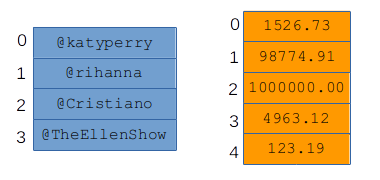
\includegraphics[width=0.6\textwidth]{array.png}
\caption{Two arrays.}
\label{fig:array}
\end{figure}

\index{index@index (pl:~indices)}
\label{arrayIndex}

Worthy of special note are the numbers on the left-hand side. These numbers
are called the \textbf{indices} (singular:~\textbf{index}) of the array.
They exist simply so we have a way to talk about the individual elements. I
could say ``element \#2 of the \texttt{followees} array'' to refer to
\texttt{@Cristiano}.

\index{zero@zero, starting at}
And yes, you noticed that the index numbers start with 0, not 1. Yes, this is
weird. The reason I did that it is because nearly all programming languages
(including Python) number their array elements starting with zero, so you might
as well just start getting used to it now. It's really not hard once you get
past the initial weirdness.

Arrays are the most basic kind of aggregate data there is, and they are the
workhorse of a whole lot of Data Science processing. Sometimes they're called
\textbf{lists}, \textbf{vectors}, or \textbf{sequences}, by the way. (When a
particular concept has lots of different names, you know it's important.)

\index{array!associative}
\index{key-value pair}
\subsection{Associative arrays}
\label{sec:assocArrays}

An \textbf{associative array}, by contrast, has no index numbers. And its
elements are slightly more complicated: instead of just bare values, an
associative array contains \textbf{key-value pairs}.
Figure~\ref{fig:assocArray} shows a couple of examples. The left-hand side of
each picture shows the keys, and the right-hand side the corresponding value.

With an associative array, you don't ask ``what's element \#3?'' like you do
with a regular array. Instead, you ask ``what value is associated with the
\texttt{"Washington"} key?'' And out pops your answer (\texttt{"Redskins"}).

\begin{figure}[ht]
\centering
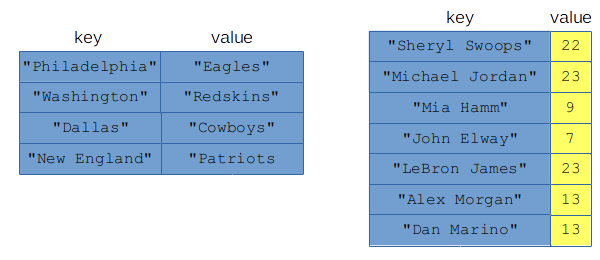
\includegraphics[width=0.9\textwidth]{assocArray.png}
\caption{Two associative arrays.}
\label{fig:assocArray}
\end{figure}

\index{order}
\index{undefined}
\index{mapping (a key to a value)}
All access to the associative array is through the keys: you can change the
value that goes with a key, retrieve the value that goes with a key, or even
retrieve and process \textit{all} the keys and their associated values
sequentially.\footnote{Using something called a ``loop,'' which we'll learn
about a little later in the book.} In that third case, the order in which
you'll receive the key-value pairs is \textbf{undefined} (which means ``not
guaranteed to be consistent'' or ``not necessarily what you'd expect.'') This
underscores the fact that there isn't any reliable ``first'' key-value pair,
or second, or last. They're just kind of all equally ``in there.'' Your mental
model of an associative array should just think of keys that are
\textbf{mapped} to values (we say that \texttt{"Dallas"} is ``mapped'' to
\texttt{"Cowboys"}) without any implied order. (Sure, the
\texttt{"Philadelphia"}/\texttt{"Eagles"} pair is at the top of the picture,
but that's only because I had to put \textit{something} at the top of the
picture, and I chose Philadelphia at random. It doesn't have any meaningful
primacy though.)

\index{homogeneous} Note a couple things about Figure~\ref{fig:assocArray}.
First, the keys in an associative array will almost always (and for us,
\textit{always}) be homogeneous. Similarly, the values will be homogeneous. But
the keys might not be of the same type as the values. In the left picture, both
keys and values are text, but in the right picture, the keys are text and the
values (uniform numbers of famous athletes) are whole numbers. This is
perfectly healthy and good.

\index{uniqueness!of keys in an associative array}
Second, realize that the \textit{keys} in an associative array must be
\textbf{unique} -- this means that there can be no duplicate keys. If we tried
to create a second \texttt{"Alex Morgan"} (oh, if only...) with a different
value, that new value would \textit{replace} Alex's current value, not sit
alongside the first one as an additional key-value pair.

The reverse is not true, however: the \textit{values} of an associative array
may very well not be unique. In the left-hand picture they are, but in the
right-hand picture there are duplicates: both Jordan and LeBron wore \#23 in
their stellar careers, while Hall of Famer quarterback Dan Marino once chose
the same uniform number that Alex wears today. This isn't a problem, because we
always access the information in an associative array \textit{through the
keys}. Asking ``what number did Mia Hamm wear?'' gives us a well-defined
answer. Asking ``which famous athlete wore \#23?'' does not. That's why we
can't ask that second question (and aren't meant to).

\subsection{Tables}

\index{table}

Lastly, we have the table, which in Data Science is positively ubiquitous. In
Figure~\ref{fig:table} we return to the pinterest.com example, with a table of
their most popular users. As you can see, it has more going on that than the
previous two aggregate data types. Still, it's pretty straightforward to wrap
your head around.

\begin{figure}[ht]
\centering
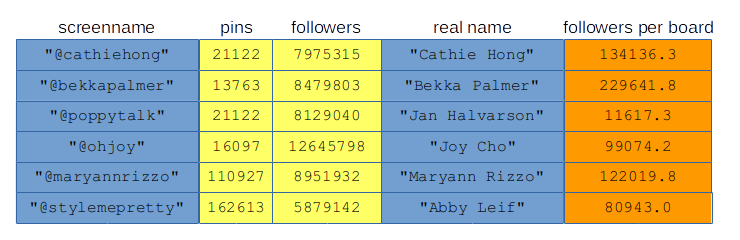
\includegraphics[width=\textwidth]{table.png}
\caption{A table.}
\label{fig:table}
\end{figure}

\index{row (of a table)}
\index{column (of a table)}
Unlike the other two aggregate data types, tables are full-on two-dimensional.
There's (theoretically) no limit to how many \textbf{rows} and how many
\textbf{columns} they can have. By the way, it's important to get those two
terms straight: rows go across, and columns go up and down. (Think of the
columns in the Trinkle Rotunda.) Also, the typical table has many, many more
rows than columns, so they're super tall and skinny, not short and fat.

\index{heterogeneous}
\index{homogeneous}
Although the \textit{rows} of a table are often heterogeneous, each
\textit{column} must be homogeneous. You can see that with a glance at
Figure~\ref{fig:table}. Each column represents a specific type of data -- in
this case, some statistic or piece of information about a Pinterest user.
Clearly all screen names should be of a text type, all ``number of pins or
followers'' should be whole numbers, \textit{etc.} It doesn't make sense
otherwise.

\index{order}
\label{assocArraysUnordered}
As with the other types, the whole dog-gone table -- no matter how many
millions of rows it might have -- is \textit{one} variable with a single name.
Also, just like with associative arrays, there normally isn't any implied
\textit{order} to the rows. Many implementations of these data types (including
Python/Pandas) will actually let you specify ``the first row'' or ``the
$53^{\textrm{rd}}$ row,'' but that always makes me cringe because conceptually,
there isn't any such thing. They're just ``rows'' that are all ``in
there.''

\subsubsection{``Querying'' tables (and other things)}

\index{query}
\label{tablesHaveNoKey}

Now you might be wondering how to actually ``get at'' the individual values of
a table. Unlike arrays, there's no index number. And unlike associative arrays,
there's no key. How then to address, say, the \texttt{@poppytalk} row?

The answer will turn out to be something called a \textbf{query}, which is a
geeky way of saying ``a set of criteria which will match some, but not all, of
the rows and/or columns.'' For instance, we might say ``tell me the pin count
for \texttt{@ohjoy}.'' Or, ``give me all the information for any user who has
more than 100,000 followers per board \textit{and} at least 20,000 pins.''
Those specific requirements will restrict the table to a subset of its rows
and/or columns. We'll learn the syntax for that later. It's a bit tricky but
very powerful.

\index{element}
By the way, it turns out we'll actually be using the concept of a query for
arrays and associative arrays as well. So strictly speaking, a query isn't just
a ``table thing.'' However, they're especially invaluable for tables, since
they're essentially the \textit{only} way to access individual elements.

\section{Aggregate data and memory pictures}

Recall from chapter~\ref{ch:memoryPictures} (p.~\pageref{fig:memoryPicture})
that the right-hand side of our memory pictures bore the label
``\textsf{Aggregate data}.'' You may have anticipated that that's where the
stuff in this chapter will live, and you're right. But there's a catch.
Remember that variable \textit{names} live on the left-hand side, and that's
true even if the variable is of an aggregate type! This turns out to be
crucially important, so I'm going to make a big deal about it.

You must draw your memory pictures (either on a whiteboard, or in your head) in
a very specific way, and that way is illustrated in
Figure~\ref{fig:aggregateMemory}.

\begin{figure}[ht]
\centering
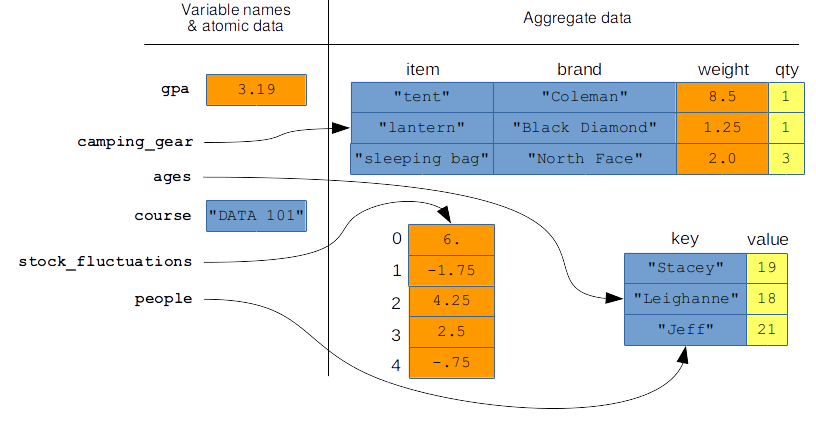
\includegraphics[width=1\textwidth]{aggregateMemory.png}
\caption{Where aggregate data variables -- and their variable names -- live in
memory.}
\label{fig:aggregateMemory}
\end{figure}

Study this picture carefully, and notice several vitally important things.
First, \textit{all} the variable names are on the left-hand side -- whether
aggregate or not. This is always, always true.

\index{pointer}
\index{reference}

Second, the actual array, associative array, and table depicted in this diagram
are on the right-hand side. The variable name on the left ``\textbf{points
to}'' the data in question with a little arrow. The technical name for this
arrow is a \textbf{pointer} or a \textbf{reference}. The rule is simple: each
atomic variable (like \texttt{gpa} or \texttt{course}) contains \textit{the
colored box itself}. Aggregate variables (like the other four) contain
\textit{a pointer to the group of colored boxes.}

Finally, mull over the fact that two \textit{different} variables in this
memory picture are pointing to the same thing! (\texttt{ages} and
\texttt{people}) Believe it or not, this is a normal occurrence. The
consequence is that if Stacey had a birthday, and we increased her age from 19
to 20 in the associative array, \textit{both} \texttt{ages} \textit{and}
\texttt{people} would automatically see the new value. There is only one copy
of that associative array in memory, and both variable names point at it.

It may seem like I'm being pedantic with this left-side-right-side stuff and
all the little arrows. \textbf{I promise you I'm not.} The moment your data
analysis program gets even mildly complicated, you will do the \textit{wrong}
thing and get the \textit{wrong} answers if you don't think of it exactly like
this. Take your time and commit it to memory.


\backmatter
\printindex

\end{document}
